This chapter introduces the fundamental concepts required to understand stateful failure tracking and resolution in modular, \gls{soa} based industrial routers. It outlines the technological background of industrial communication networks and routers, explains Service-Oriented Architecture in this context, defines faults and failures in service-based systems, describes telemetry and observability, discusses service dependencies and failure propagation, and summarises core principles of Fault Detection, Isolation and Recovery (\gls{fdir}). The chapter concludes with router specific constraints that influence the design of any fault management framework. Together, these foundations provide the conceptual basis for the research questions and approach developed in subsequent chapters.

\section{Industrial Communication Networks and Routers}

Industrial communication networks support data exchange among field devices, controllers, supervisory systems, and higher-level \gls{it} infrastructures. Typical examples include production lines, process plants, energy distribution networks, and transportation systems including rail and road vehicles that rely on cellular connectivity for remote management. In these environments, communication infrastructures operate under strict requirements regarding availability, timing behaviour, determinism, and safety. Interruptions can affect any network component cables, power supplies, wireless links subject to interference, or the routers themselves and propagate to dependent applications.

Industrial routers occupy a central position in these networks. They interconnect different subnetworks, bridge between operational technology (\gls{ot}) and information technology (\gls{it}), and provide security, remote access, and device management functions. In contrast to purely \gls{it}-focused routers, industrial routers integrate hardware and software designed for long-term deployment, extended temperature ranges, and operation in electromagnetically noisy or physically exposed environments. Configuration interfaces, device management functions, and monitoring capabilities are typically tailored to industrial use cases and to integration with \gls{scada} systems or similar platforms.

While industrial routers share core networking functions with \gls{it} routers (routing, firewalling, \gls{vpn}), the distinguishing characteristic is the operational context: industrial routers must maintain these functions under the constraints described in Section 2.7 (resource bounds, determinism requirements, long deployment lifecycles, harsh environments, safety relevance). From a functional perspective, industrial routers typically provide:

\begin{itemize}
\item L3 routing and network address translation,
\item \gls{vpn} termination,
\item firewalling and access control,
\item device and configuration management,
\item diagnostics and telemetry export.
\end{itemize}

Industrial automation applications depend on these functions primarily at the Ethernet level (OSI Layer 2) and the \gls{ip} level (OSI Layer 3). Faults affecting router functions therefore propagate beyond the network layer and directly influence application-level behaviour, production continuity, safety, and regulatory compliance. As a result, failures in industrial routers cannot be treated as isolated component faults but must be detected, analysed, and resolved with awareness of their systemic impact.

\begin{figure}[htbp]
  \centering
  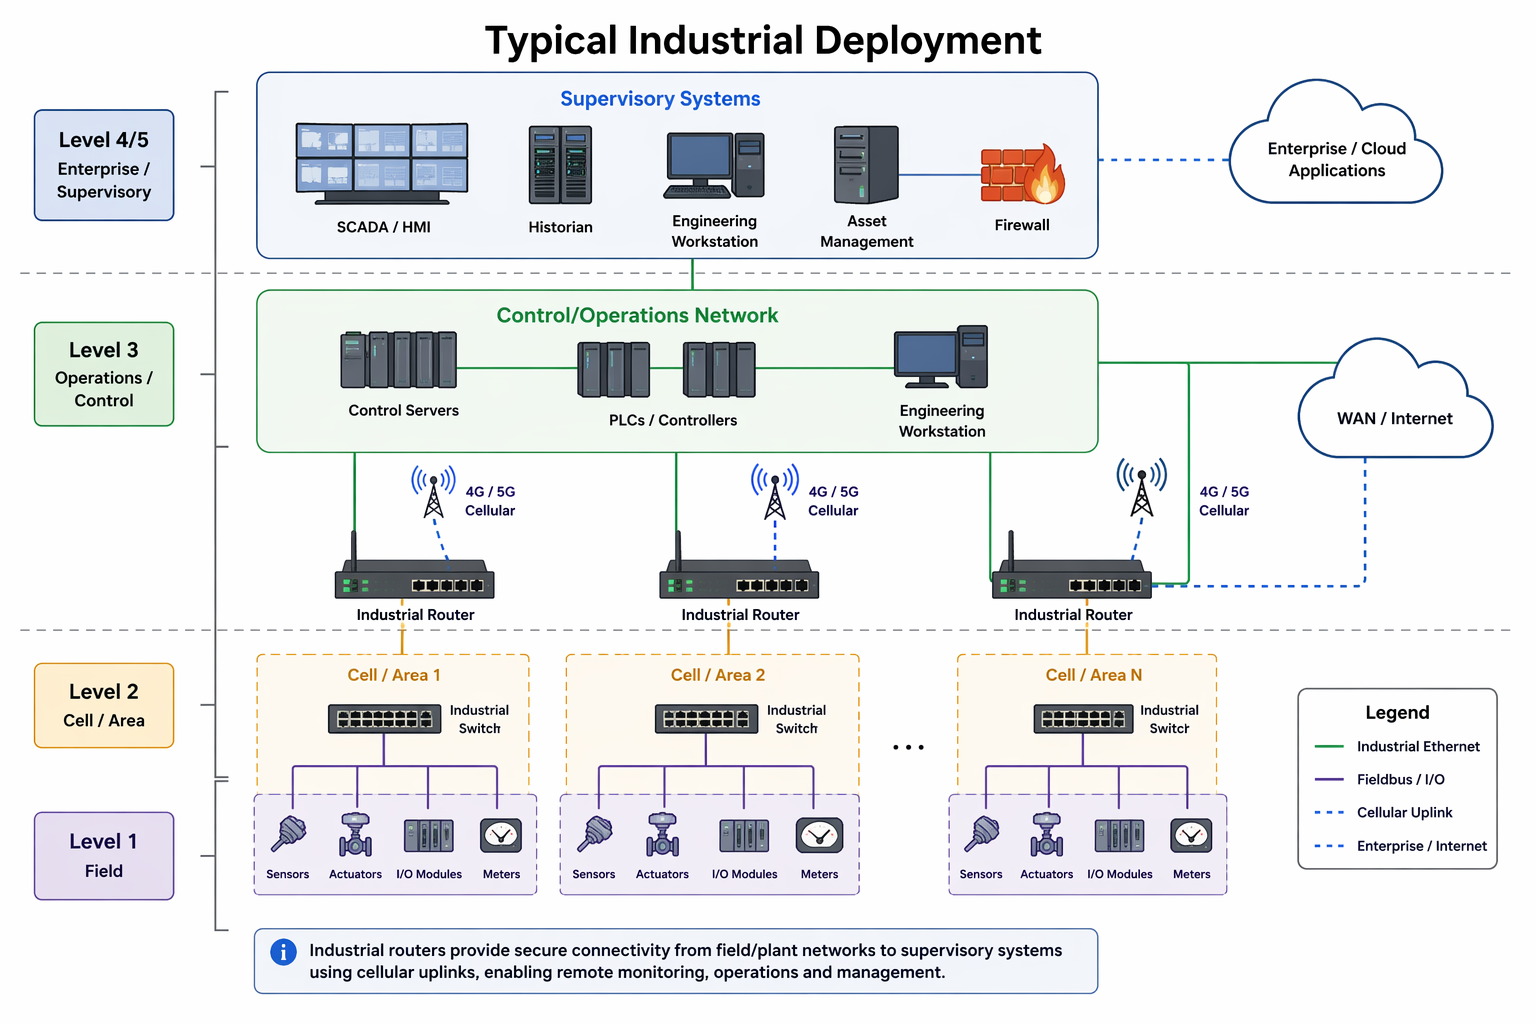
\includegraphics[width=\textwidth]{figures/typical-industrial-deployment.png}
  \caption{Typical industrial deployment}
  \label{fig:typical-industrial-deployment}
\end{figure}

\section{Service-Oriented Architecture in Industrial Routers}

Service-Oriented Architecture (\gls{soa}) is an architectural paradigm in which system functionality is decomposed into discrete services that interact through well-defined interfaces and protocols. A service encapsulates a coherent set of responsibilities, maintains its own internal state, and exposes operations to other services or clients. Service interactions rely on explicit contracts regarding inputs, outputs, and quality attributes.

In the context of industrial routers, \gls{soa} principles appear in the modularisation of router functions. \gls{vpn} management, firewall rule processing, routing table handling, certificate management, logging, and supervisory control are often implemented as separate services. These services communicate through message buses, remote procedure calls, or shared configuration stores. The resulting architecture promotes modularity, reuse, and independent evolution of components. It also enables integration of third-party services or domain specific extensions.

The adoption of \gls{soa} in embedded router platforms introduces service-based failure modes that do not exist in monolithic architectures. In a monolithic system, faults are confined within a single process boundary. In an \gls{soa} system, interface mismatches, inconsistent state between services, failures in service discovery, or timeouts in inter-service communication influence router behaviour even when individual software modules operate within their local design assumptions. A service does not need to know the internal state of another service, but it depends on the correctness of the other service's externally observable behaviour. A structured view of services, their contracts, and dependencies is therefore a prerequisite for systematic fault management in \gls{soa}-based routers.

\section{Faults, Errors, and Failures in Service-based Systems}

Fault management research distinguishes between faults, errors, and failures. A fault denotes an underlying defect or abnormal condition in a system component, such as a software bug, misconfiguration, or hardware malfunction. An error represents a system state in which some internal data or control flow deviates from the specified behaviour. A failure occurs when the delivered service deviates from its specification as perceived by an external observer.

In \gls{soa} based systems, faults arise both at the level of individual services and at the level of service compositions. Typical fault types include:

\begin{itemize}
\item interface faults (e.g.\ incorrect parameter types or missing fields),
\item communication faults (e.g.\ timeouts, connection drops, protocol violations),
\item state management faults (e.g.\ inconsistent configuration, stale caches),
\item resource faults (e.g.\ memory exhaustion, thread pool depletion),
\item orchestration faults (e.g.\ incorrect execution order, missing compensation logic).
\end{itemize}

A fault in one service produces errors in its internal state or outputs, and these errors propagate along service calls or event flows. When such propagation reaches a service boundary, external clients observe failures such as unresponsive management interfaces, dropped \gls{vpn} connections. Systematic failure analysis therefore requires a clear classification of faults and an understanding of how they manifest in observable behaviour.

For industrial routers, misconfigurations, software defects, and resource exhaustion in core services directly influence connectivity, security enforcement, and monitoring. A router specific view on fault types, including networking and industrial protocol aspects, is essential for precise fault tracking and meaningful recovery strategies.

\section{Telemetry and Observability}

Telemetry in distributed systems comprises all data that describes system behaviour and state over time. Modern observability practice often groups telemetry into three categories: metrics, logs, and traces.

Metrics represent numerical measurements sampled at defined intervals. Typical examples in routers include \gls{cpu} utilisation, memory usage, interface counters, packet drops, connection counts, and latency statistics. Metrics support trend analysis, threshold based alerting, and compact representation of long-term behaviour.

Logs record discrete events, status messages, and diagnostic information. Logs range from low level system messages to application-level events such as configuration changes, session establishment, or error reports. Structured logging formats facilitate automated processing, correlation, and filtering.

Traces capture end to end execution paths of individual requests or workflows across multiple services. A trace associates a unique identifier with a sequence of operations, including timing information and causal relationships between services. In \gls{soa} based routers, traces describe, for example, how a configuration request traverses authentication, validation, persistence, and notification services.

Observability emerges when telemetry provides sufficient insight to explain why the system behaves in a certain way, to localise root causes of failures, and to validate recovery actions. For industrial routers, telemetry generation and processing must respect resource limitations and real time constraints. Any \gls{fdir} framework for industrial routers requires a structured telemetry model that maps relevant metrics, logs, and traces to fault types and to the internal states of router services.

\section{Service Dependencies and Failure Propagation}

Service based systems exhibit complex dependency structures. A service depends on other services for data, configuration, authentication, or infrastructure access. These dependencies form directed graphs in which nodes represent services and edges represent dependency relations. Dependencies may be static, defined by configuration or design time bindings, or dynamic, created at runtime based on discovery, load balancing, or failover mechanisms.

Failure propagation in such graphs occurs when an error in one service influences the behaviour of dependent services. Examples include:

\begin{itemize}
\item a malfunctioning configuration service that provides inconsistent parameters to multiple consumers,
\item an overloaded logging service that delays or drops log messages required for monitoring and alerting,
\item an authentication service that rejects valid requests and thereby affects management, supervisory, or user facing functions.
\end{itemize}

In industrial routers, dependency structures often involve core services such as routing, \gls{vpn}, firewalling, and device management, as well as auxiliary services such as logging, certificate management. Explicit modelling of these dependencies enables reasoning about which services are potentially affected by a given fault and where to localise the root cause of an observed failure. A stateful \gls{fdir} framework therefore requires both a representation of dependency graphs and mechanisms to update these graphs when services are added, removed, or reconfigured.

\section{Fault Detection, Isolation, and Recovery (FDIR)}

Fault Detection, Isolation, and Recovery (\gls{fdir}) denote an integrated process widely used in safety-critical and mission-critical systems.

Fault detection identifies abnormal conditions through deviations from expected behaviour. Fault isolation maps observed symptoms to specific components or services, establishing the root cause or a minimal set of plausible causes. Fault recovery applies corrective actions to restore correct service behaviour, such as reconfiguration, restart, failover, or controlled degradation.

Stateful \gls{fdir} extends this process by maintaining explicit runtime information about fault episodes, recovery attempts, and current system state. This information enables the framework to distinguish between new fault occurrences and ongoing violations, to prevent redundant recovery actions, and to avoid oscillations between failure and recovery states.

In \gls{soa}-based industrial routers, stateful \gls{fdir} must integrate fault classification, telemetry interpretation, and dependency reasoning while ensuring deterministic execution, bounded resource usage, and transparent decision-making. Recovery actions must be coordinated with identified root causes and executed at most once per fault episode, while dependent symptom faults are managed in a controlled manner. These requirements go beyond stateless alerting and form the foundation for predictable and analysable fault management in embedded router platforms.

\section{Constraints and Characteristics of Industrial Routers}

Industrial routers differ from general purpose cloud or datacentre systems along several dimensions that strongly influence fault management strategies:

\begin{itemize}
\item Resource constraints: Router platforms usually integrate embedded processors and memory budgets selected for networking workloads rather than for compute intensive analytics. Telemetry capture, storage, and processing therefore require carefully bounded resource usage.
\item Realtime and determinism requirements: Communication behaviour often adheres to timing constraints imposed by industrial control loops and safety systems. Fault detection and recovery mechanisms must avoid unpredictable delays and must preserve deterministic routing and forwarding behaviour.
\item Long deployment lifecycles: Industrial routers operate in the field over extended periods, with infrequent maintenance windows. Fault management mechanisms must accommodate incremental software updates, heterogeneous firmware versions, and constrained opportunities for human intervention.
\item Harsh environmental conditions: Temperature variations, electromagnetic interference, and physical stress influence hardware reliability and increase the likelihood of faults in interfaces, power supply, or storage media.
\item Safety and security relevance: Routers often form part of safety related communication paths and serve as security gateways between \gls{ot} and \gls{it} networks. Incorrect fault handling affects both functional safety and cybersecurity posture.
\item Operational predictability and certification requirements: Fault management behaviour must be analysable, explainable, and reproducible across deployments. Recovery logic must avoid nondeterministic decision-making and uncontrolled repetition, supporting certification and long-term maintenance.
\end{itemize}

These characteristics require fault management approaches that favour deterministic logic, explicit state tracking, transparent decision-making, and bounded use of telemetry over heavyweight, data-driven methods. An \gls{fdir} framework for industrial routers must therefore incorporate stateful fault episode management, dependency-aware recovery coordination, and bounded execution semantics, while remaining adaptable to evolving service architectures and operational requirements. The framework presented in Chapter 5 addresses these constraints as follows: resource constraints are addressed through a bounded event queue and sample-driven processing (Principles 1 and 5); determinism is addressed through single-threaded, deterministic rule evaluation with no \gls{ml}-based inference (Principle 2); long deployment lifecycles are addressed through declarative \gls{yang}/\gls{netconf} configuration that supports runtime reconfiguration without code changes (Principle 3); harsh environmental conditions are addressed indirectly the framework detects their effects through telemetry symptoms but does not manage hardware faults directly (Section 5.1.3); and safety/security relevance is addressed through root-cause-only resolution that prevents cascading recovery actions from disrupting the forwarding plane (Principle 4). The next chapter formulates the research questions and outlines the methodology used to investigate stateful failure tracking and recovery in industrial routers.